\subsubsection{Post-absorptive and fasting state}
\label{sec:PostAbsorptiveAndFastingState}

The four-hour to six-hour interval following ingestion of a meal is generally referred to as the post-absorptive state. At this point, plasma glucose concentrations average 80 to 90 mg/dl, and rates of glucose utilization are approximately 2 mg/kg/min. At least 50\% of whole body glucose utilization is due to noninsulin-dependent uptake of glucose from the brain. The formed elements of the blood, renal medulla and muscle, metabolize glucose to pyruvate and lactate.  These substances can be released into the circulation and serve as substrates for gluconeogenesis. In the postabsorptive state, insulin sensitive tissues such as muscle, adipose tissue, and liver account for less than 30\% to 50\% of overall glucose utilization. Following meal ingestion, however, liver and muscle take up glucose to replenish their glycogen stores and transiently increase their utilization of glucose.

If fasting is prolonged beyond the post-absorptive period, plasma glucose concentrations decrease over the succeeding 48 to 78 hours to reach a nadir of approximately 45 to 60 mg/dl that can be maintained for several weeks. Plasma free fatty acids and ketone body concentrations increase several-fold, reaching levels of 1 to 2 mmol/l by 72 hours. Glucose utilization decreases during this time to approximately 1 mg/kg/min and remains constant thereafter. These changes are in large part due to decreases in plasma insulin concentration that permits accelerated lipolysis with increased ketone body formation. Muscle and other tissues become progressively more dependent on free fatty acids and ketone bodies. Also, ketone bodies replace glucose as the predominant fuel for neural tissues, thus reducing the obligatory glucose uptake by the brain.

\subsubsection{Absorptive state}
\label{sec:AbsorptiveState}

The increase in plasma insulin concentration that occurs immediately following a meal suppresses endogenous glucose production, an effect also mediated by the increased plasma glucose concentration. Consequently, hepatic glycogenolysis is suppressed and glycogen deposition stimulated. Approximately 50\% of an oral glucose load is taken up by the liver and the remaining by peripheral insulin-sensitive tissues. Three to four hours following meal ingestion, the liver again releases glucose into circulation. Ultimately, the rate of glucose released equals the rate of glucose utilization so that plasma glucose concentrations are maintained stable.

Nearly all tissues, to varying degrees, oxidize glucose to derive energy for metabolic demands. Yet only the liver and kidney release glucose. This release results from the presence in these organs of glucose-6-phosphatase which liberates glucose into the bloodstream. The liver and kidney do not, however, contribute equally to post-absorptive glucose homeostasis. It is generally believed that the liver makes the major quantitative contribution during this state, while the kidney plays a minor role. 

\section{Diabetes Mellitus}
\label{sec:DiabetesMellitus}

For 2,000 years diabetes has been recognized as a devastating and deadly disease. In the first century A.D. a Greek, Aretaeus, described the destructive nature of the affliction which he named ``diabetes'' from the Greek word for ``siphon''. Eugene J. Leopold in his text Aretaeus the Cappodacian describes Aretaeus' diagnosis: ``...For fluids do not remain in the body, but use the body only as a channel through which they may flow out. Life lasts only for a time, but not very long. For they urinate with pain and painful is the emaciation. For no essential part of the drink is absorbed by the body while great masses of the flesh are liquefied into urine''.

Physicians in ancient times, like Aretaeus, recognized the symptoms of diabetes but were powerless to effectively treat it. Aretaeus recommended oil of roses, dates, raw quinces, and gruel. And as late as the 17th century, doctors prescribed ``gelly of viper's flesh, broken red coral, sweet almonds, and fresh flowers of blind nettles''.

In the 17th century a London physician, Dr. Thomas Willis, determined whether his patients had diabetes or not by sampling their urine. If it had a sweet taste (due to a phenomenon known as glycosuria, which occurs when blood glucose goes up above the threshold of 180 mg/dl) he would diagnose them with diabetes mellitus- ``honeyed'' diabetes. This method of monitoring urine glucose went largely unchanged until the 20th century.

In the early 20th century, diabetologists such as Dr. Frederick Allen prescribed low calorie diets-as little as 450 calories per day for his diabetic patients. His diet prolonged the life of people with diabetes but kept them suffering from near starvation. In effect, people with diabetes suffered a painful wasting death. Then in 1921 something truly revolutionary occurred in Ontario, Canada. A young surgeon Frederick Banting, and his assistant Charles Best, kept a severely diabetic dog alive for 70 days by injecting it with a murky concoction of canine pancreas extract. With the help of Dr. Collip and Dr. Macleod, Banting and Best administered a more refined extract of insulin to Leonard Thompson, a young boy dying of diabetes. Within 24 hours, Leonard's dangerously high blood sugars had dropped to near normal levels. Until the discovery of insulin, most children diagnosed with diabetes were expected to live less than a year. In a matter of 24 hours the boy's life had been saved. News of the miracle extract, insulin, spread like wildfire across the world.

Since insulin's discovery, medical breakthroughs continued to prolong and ease the lives of people with diabetes. In 1935 Roger Hinsworth discovered there were two types of diabetes: ``insulin sensitive'' (type 1) and ``insulin insensitive'' (type 2). By differentiating between the two types of diabetes, Hinsworth helped open up new avenues of treatment. Indeed, type 1 and type 2 diabetes are characterized by different pathophysiologic processes, resulting in different therapeutical approaches. 


There are two main types of diabetes mellitus. Type 1 diabetes is characterized by absolute insulin deficit, due to the autoimmune destruction of the pancreatic beta cells. Hence, the treatment for people with type 1 diabetes is necessarily the replacement of the endogenous insulin secretion by means of the administration of exogenous insulin. On the other hand, type 2 diabetes is the result of two concomitant alterations: 1) insulin resistance (i.e. the liver and the muscle have less than normal sensitivity to the insulin action); 2) impaired beta cell function (i.e. the physiological response of the beta cell to a meal is lost, as well as its ability to compensate for insulin resistance). This results in relative insulin deficit, which can be approached with several non pharmacological (physical exercise) and pharmacological measures. However, the natural history of type 2 diabetes is characterized by progressive lost of the beta cell function overtime, finally leading to a condition of absolute insulin deficit requiring replacement with exogenous insulin.

There are other types of DM, like the pathologies that are induced by infections or endocrinopathies, and they can be of transitional character, like the gestational diabetes occurring in pregnant women, or remain chronic for the patient, but these sorts of DM are not going to be studied in here. Diabetes type 1 and 2 will be explained in detail in chapters \ref{sec:DiabetesType2} and \ref{sec:DiabetesType1}.

The degree of metabolic control obtained by people with diabetes can be measured by the concentration of \textit{glycated hemoglobin} in blood, also called \textit{HbA1c}. Hemoglobin is the protein used to transport oxygen though the circulatory system. In presence of glucose it undergoes a non-enzymatic reaction, becoming glycated. This transformation is in relation to the average concentration of glucose in blood, due to the half-life of red blood cells, it is representative of mean blood glucose concentrations during the past 8-12 weeks. For the record, a healthy person has a 5.5\% of hemoglobin in glycated state, while a diabetic patient is considered to be under control if its HbA1c is under 7\%.

\subsubsection{Current strategies for insulin replacement}
\label{sec:CurrentStrategiesForInsulinReplacement}

In the early 1980s human insulin was introduced to the market by drug companies substituting animal insulin emphasizing the belief that diabetic people should be treated with ``naturally'' secreted insulin from the human body. Better glycaemic control was expected in people with diabetes using human compared with animal insulin. This was not the case, since no single advantage could be proven for humans versus animal insulin (\cite{sonnenberg1983human}).

However, the positive aspect of human insulin was the innovative technology used for its production (DNA-recombinant technique) versus the traditional insulin extraction method from animal pancreata. This new technique helped to develop a number of insulin analogues. Major efforts were started to modify the human insulin and develop ``modified'' insulins for administration to diabetic subjects. Slow and rapid acting insulin analogues are available now for the different stages of the treatment of diabetes. Slow acting insulins (up to 24h permanence in blood) can be used for substituting the flat insulin level in the interprandial periods. Fast acting insulin analogues (1-2 hours life cycle) on the contrary, may be used to replicate the postprandial insulin peaks of the (non-existent) insulin secretion.

Regardless of the system of glucose measurement or the way insulin is delivered, the control philosophy for glucose control in DM1 is to replicate the insulin secretion pattern of the non-diabetic person. As already explained, in the fasting and post-absorptive state, insulin secretory rate is regulated in a feedback fashion by plasma glucose levels. This is known as \emph{basal insulin}, which modulates hepatic glucose production to exactly compensate for peripheral glucose utilization maintaining plasma glucose concentrations in a very narrow range. In the post prandial state, beta cells increase insulin secretion to cope with glucose absorption from the gut into the bloodstream. This is called \emph{prandial insulin} secretion, which results in high plasma insulin concentrations that suppress hepatic glucose production (unnecessary since glucose is being absorbed from the gut) and increase glucose disposal into the liver and the muscle, allowing for very small meal-induced fluctuations in plasma glucose concentrations. It should be noted that the feedback mechanisms regulating insulin secretion, probably rely on measurement of glucose concentration in the blood (or in some compartment in fast equilibrium with the blood). Thus, mimicking physiological insulin secretion must translate into replacement of both basal and prandial components, and ideally it should be based on measurements of blood glucose concentrations and on insulin infusion directly into the blood stream. %Usually, after eating, in a healthy person there is a rapid increase in plasma insulin, called \textit{bolus}, which copes with postprandial glycaemia by stimulating peripheral glucose uptake. During the rest of the day, plasma insulin is forced to be stable to a level that restrains plasma glucose to normoglycaemia. Those levels, both of glucose and insulin are called \textit{basal} concentrations, or if talking about dosages, basal supplies.%

However, for practical reasons in clinical practice, insulin is usually injected subcutaneously. This introduces a delay between insulin injection and insulin action, which represents the time needed for the absorption of insulin from the subcutaneous tissue into the blood. This lag time depends on the chemical properties of the insulin injected (which influence its rate of absorption) and  is one of the barriers to the development of the artificial pancreas. The insulin molecule has been modified in order to obtain preparations suitable for more accurate insulin replacement (\cite{rossetti2008superiority}). Indeed, current strategies for insulin administration use a long-acting insulin analogs (the molecule has been modified to ensure a constant 24 hour absorption from the subcutaneous tissue, following injection) for basal replacement and a fast acting insulin analogs (the molecule has been modified to accelerate its absorption from the subcutaneous tissue) for prandial requirements. This therapy is called \emph{basal-bolus} strategy, and it is clearly limited by the pharmacokinetics of insulin, and leaves no possibility of reaction to unexpected events, such us too low absorption rate of glucose, or sudden increase of insulin sensitivity of the patient.

\begin{figure}[hbtp]
\centering
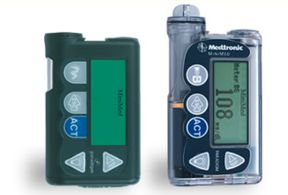
\epsfig{file=Figures/pumps.jpg, width=0.6\textwidth}\caption{Insulin pumps \cite{medtronic}}
\label{fig:pumps}
\end{figure}

Subcutaneous insulin pumps (as shown in figure \ref{fig:pumps}) traditionally use basal-bolus strategy, but the possibility of adjusting the insulin delivery rate at any time rises scenarios of a closer control. The main advantages of using Continuous Subcutaneous Insulin Infusion (CSII) are:
\begin{enumerate}
	\item Use of rapid acting analogs both for meal insulin and basal insulin. Indeed, they show better reproducibility of subcutaneous absorption as compared to long acting insulins resulting in lower variability.
	\item Possibility to adjust basal insulin requirements to the subject needs (ex circadian variations in insulin sensitivity). This is not possible with long acting insulins with `fixed' pharmacokinetics and pharmacodynamics.
\end{enumerate}

These new CSII scenarios require of a more efficient glucose measuring system as well, and the recent subcutaneous real-time glucose monitors, like the guardian real-time glucose monitoring system from Medtronic shown in figure \ref{fig:guardian}, provide this continuous monitoring required to close the control loop.

\begin{figure}[hbtp]
\centering
\epsfig{file=Figures/guardian.jpg, width=0.8\textwidth}\caption{Guardian Real-Time Glucose Monitoring System from Medtronic \cite{medtronic}}
\label{fig:guardian}
\end{figure}

Given the chance to read glucose in real-time and act over it with (at least) one control action, which is the insulin infusion, it is defined a control system, and there are several control laws that can be applied to create a tighter control of blood glucose than trying to mimic the behavior of the physiological insulin production rate. The ``natural'' physiological control is impossible to obtain with the subcutaneous infusion of insulin. However, the presence of continuous sensors, even though the uncertainty that present, opens the possibility of designing new control strategies that will stabilize glycaemia in diabetic patients.

Even though the simplifications performed to the ``real'' model are strong, a reliable control law can be implemented and tested in real patients. This control problem has been a matter of research for over 40 years, and it is still going on. The product that is edxpected from the design and implementation of the control law that is to replace the damaged $\beta$-cells in the pancreas is called \textit{Artificial Pancreas}, and it is the framework of research this thesis is placed in.

\section{Artificial Pancreas}
\label{sec:ArtificialPancreas}

Over the last 30 years, even with the availability of new insulin preparations with more physiological profiles, continuous administration systems aimed at emulating endogenous insulin secretion, and new education strategies, there is still no universal, efficient and safe system able to normalize the glucose levels of diabetic patients. Progress with enzyme electrodes in the 1970s \cite{williams1970electrochemical} allowed for the emergence of continuous glucose monitoring (CGM), and for the subsequent development of the first prototypes of glucose-sensor controlled insulin infusion systems, by different groups (\cite{albisser1974artificial} and  \cite{albisser1974clinical}). 

The next two decades saw huge progress in the development of continuous glucose sensing. Research focused on the skin as an appropriate candidate for direct glucose measurement. Indeed, the subcutaneous tissue is easily accessible for sensor implantation and measurement of glucose in the interstitial fluid, with fewer problems as compared to the intravascular space. The amperometric glucose-sensing technique was refined and this process culminated, in 1999, with the development and FDA approval of the CGMS? the first commercial CGM device \cite{mastrototaro2000minimed}. Since then, technological progresses have fueled research on closed-loop glucose control systems using the subcutaneous route (see below), for effective treatment of diabetic subjects. 

Preliminary studies using off-the-shelf insulin pumps and subcutaneous continuous glucose monitoring (CGM) sensors have suggested that, in research settings, closed-loop systems that automatically dispense insulin can achieve better control of glucose levels than open-loop systems in which a person makes dosing decisions \cite{steil2006feasibility}. Such promising results prompted the Juvenile Diabetes Research Foundation (JDRF) to push the research forward by launching its Artificial Pancreas Project 4 years ago, and the US Food and Drug Administration (FDA) to designate the artificial pancreas as a priority within its Critical Path Initiative. However, so far only a few prototypes have been developed and tested in controlled clinical settings. In fact, several challenges do still exist:
\begin{enumerate}
	\item Coping with big disturbances affecting the system, such as meals, stress and exercise
	\item Robustness face to the great variability of patient's physiological behavior
	\item Accuracy and reliability of continuous glucose monitors, that must be improved to a higher degree
	\item Safety of insulin pumps and detection of faults
	\item Adequate correction for the slow responsiveness of controllers due to delays in the control loop (see below)
\end{enumerate}

Control of post-prandial glycaemic excursions is certainly a key issue in the artificial pancreas. Indeed, meals are one of the major perturbations to counteract and the main challenge found in current clinical validations of the few existing prototypes of closed-loop glycaemic control systems. This thesis focus on this issue, aiming at the development of new feedback strategies for post-prandial glycaemic control. 

%For the last 20 years there has been an unprecedented technological development in the glucose continuous monitoring area, resulting in the first generation of glucose monitors for patient use, and not only for research purposes. There are many research projects working in different areas of the artificial pancreas, for the behavior of the human glucose regulatory system is not always the same. There is, for example, the need of control in the critically ill patients that are under very strict requirements of metabolic control of glucose, and their behavior against insulin or other drugs is much different than diabetic patients. Kondepati\cite{kondepati2007recent} gives a review of this research branch in detail.

%In this thesis the effort is focused in diabetic patient control, and its postprandial (after a meal) control, and in next chapters a picture of the current development of closed loop control for this kind of patients is displayed.

\subsection{Current state of development}
\label{sec:Currentstateofdevelopment}

The first experiment conducted closing the control loop in a patient with diabetes can be traced back to 1964 by Kadish \cite{kadish1963automation}. It was the first trial to control the blood glucose with a continuous glucose monitor, and the control algorithm was just an `on-off' system with constant supervision of doctors, and the control action (insulin) was delivered in an intravenous way, which minimizes the delays related to insulin transport in tissues. 

In 1974 an `artificial endocrine pancreas' was developed simultaneously by two different researchers, Albisser \cite{albisser1974artificial} and Pfeiffer \cite{pfeiffer1974artificial}, which led to the first commercial device that emulated an artificial pancreas: The Biostator. The device implemented a complex algorithm aiming to prevent postprandial hyperglycaemia, but it was still a bulky machine (figure \ref{fig:biostator}) with need of constant supervision and none at all designed for an independent use.

\begin{figure}[hbtp]
\centering
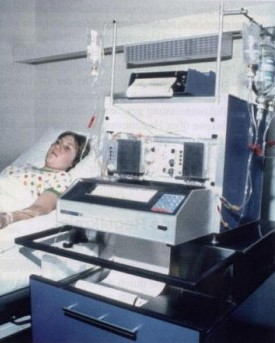
\epsfig{file=Figures/biostator.jpg, width=0.6\textwidth}\caption{Biostator designed by Pfeiffer \cite{pfeiffer1974artificial}}
\label{fig:biostator}
\end{figure}

As already said, considerable improvement has been made in the technology of glucose monitors for the past 20 years, and insulin pumps have been developed and proven to be reliable and to improve life quality for diabetic patients, as shown by Pickup \cite{pickup2002continuous}. The use of continuous insulin infusion coupled with subcutaneous aims to solve the main problem the Biostator supposed, its low manageability, but it adds new delays to the control loop, which makes the algorithms needed much more complicated.

The classification of closed-loop systems based on the body interface, and thus related to its average delay stays as follows:
\begin{itemize}
	\item \textbf{Intravenous measuring and intravenous insulin delivery.} This option is the most invasive system, and it represents the minimum delay possible from the glucose measuring to its response (about 30 minutes). A revision of the control algorithms used in this paradigm was done by Parker \cite{parker2001intravenous}. Its application is unfeasible in clinical practice and might be used, in the near future, only in critical patients and hospital treatments (in contexts where invasive techniques do not constitute a barrier to its implementation). The Biostator is the main example for this sort of interface.
	\item \textbf{Intravenous measuring and intraperitoneal insulin delivery.} Implantable insulin pumps have been used for intraperitoneal (into the abdominal cavity) infusion, which has many of the advantages of the full-intravenous interface. However, it still is invasive and adds the delay related to the absorption of the insulin.
	\item \textbf{Subcutaneous measuring and subcutaneous insulin delivery.} It is the less invasive option but also the choice that adds the largest delays to the control loop. This system is the more suited for long time treatments, and is the one that is going to be studied in detail in this thesis.
\end{itemize}
The increasing delay added by the less invasive interfaces is a present problem anytime designing a controller for blood glucose. Revision of the main drawbacks and advantages for every method was done by Hovorka \cite{hovorka2006continuous}, and the delays present in every sort of control system can be seen in figure \ref{fig:delays}.

\begin{figure}[hbtp]
\centering
\epsfig{file=Figures/delays.jpg, width=0.9\textwidth}\caption{Delays related to the interface of the artificial pancreas system as stated by Hovorka \cite{hovorka2006continuous}. s.c. stands for the subcutaneous route, i.p. stands for the intraperitoneal route and i.v. stands for the intravenous interface.}
\label{fig:delays}
\end{figure}

Other possible classification for closed-loop control in diabetes will be regarding the control algorithm implemented:
\begin{itemize}
	\item \textbf{PID control.} The classical approach control of Proportional-Integral-Derivative (PID) control is the broadest implemented control algorithm in industrial applications due to its simplicity and the fact that tuning algorithms for the controller have been developed for decades.
	\begin{equation}\label{eq:PIDcontrol}
			IIR = K_{p}(G-G_{t}) + K_{I}\int(G-G_{t}) + K_{d}\frac{\partial G}{\partial t}
	\end{equation}
	Where $IIR$ represents the insulin infusion rate, $K_{p}$, $K_{d}$ and $K_{i}$  are the parameters of the controller (to be determined), $G$ is the measured glucose, and $G_{t}$ is the target glucose. Due to its simplicity, many times the PID gives the base structure to the controller, and many heuristic methods make the controller an ``expert'' controller. Marchetti \cite{marchetti2008improved} for example, developed one of these algorithms for type 1 diabetic patients and Chee \cite{chee2003expert} did it for critically ill patients.
	\item \textbf{State-feedback control.} The so called ``Optimum control'' methodology has been used to design algorithms as a feedback of the state of the model considered. Palumbo \cite{palumbo2008robust}, for example, used this approach to design a controller for a Delayed Differential Equation model of the glucose regulation system.
	\item \textbf{Model predictive control (MPC).} MPC is a rather more complex control philosophy, based on optimization methods to find the optimum input that leads the controlled variable to the desired reference in a target time. It is, as well as the PID controller, widely implemented in industries, and the tuning algorithms are very efficient and have been refined for the last decades. A complete overview for the development of the algorithm and its impact on industry was performed by Camacho and Bordons \cite{camacho2004model}. In the context of artificial pancreas MPC is the  most applied method of control, and several controllers have been developed, such as the one of Parker \cite{parker1999model}, or the one implemented by Hovorka \cite{hovorka2004nonlinear}, which was tested in its application on critical patients by Plank \cite{plank2006multicentric}, showing that patients were more often within the glucose target range than with the usual therapy, and that hypoglycemia episodes were avoided completely by using the MPC controller.
\end{itemize}
About the optimum algorithm to be chosen in order to control a determined patient, the answer is not clear. Despite MPC methodology has been the most used option, it is mathematically proven that if the model is close enough to reality, the feedback of the state is the most robust and fastest control possible. That raises the question of whether the models used are reliable or useful, and how much should we deepen in the matter of modeling, or just use impulse and step models, as many MPC controllers do. The question of modeling is explained in depth in chapter \ref{sec:ModelingInDM1}.

The last classification of artificial pancreas systems is regarding the situation of the patient during the control, or the population that the system aims to control:
\begin{itemize}
	\item \textbf{Pregnant woman transitional diabetes.} Gestational diabetes has been studied from the point of view of artificial pancreas in several works. Murphy et al. \cite{murphy2008effectiveness} showed the effectiveness of continuous glucose monitoring in pregnant women with diabetes, and Hernando et al. \cite{hernando1996diabnet} used algorithms based in diabetic models to plan insulin therapy. No specific controllers have been designed for this particular case.
	\item \textbf{Critical patient control.} Critical patients are monitored in detail, not only in glucose, but also in many other important measures of body functions, which are intended to be as controlled as possible. This fact gives the opportunity to test many controllers designed for glucose regulation. The previously mentioned controller of Chee et al. \cite{chee2003expert} and the one designed by Hovorka's group in Cambridge \cite{plank2006multicentric}, are examples of controllers used to maintain the glucose homeostasis in intensive care unit patients.
	\item \textbf{Overnight fasting control.} Overnight period is usually related to a natural reduction of the sensibility to insulin, and the lack of consideration of this effect creates an increase in blood glucose that is commonly known as ``Dawn effect''. Hovorka's group, for example, has achieved great success in controlling this kind of behavior by means of glucose monitoring and MPC controllers both with subcutaneous and intravenous interfaces \cite{schaller2006line}.
	\item \textbf{Postprandial control.} The main disturbance to blood glucose control is the absorption of glucose from the gut. The postprandial blood glucose control aims to soften the abrupt increase of glucose after a meal without risking the patient's health. This thesis will be focused in this kind of control, which will be explained in detail in chapter \ref{sec:Postprandialcontrolofmixesmodels}.
\end{itemize}
Despite all the work that has been done already, the practical realization of a human pancreas is not yet possible, nor implanted as an artificial organ due to maintenance issues, neither emulated by an external device. The main problem with the external approach, as stated by Hovorka \cite{hovorka2006continuous}, is the low reliability and exactitude of the subcutaneous continuous glucose monitors, assuming the subcutaneous (and more comfortable to the patient) interface. Work has yet to be done in this area principally about characterizing the monitor behavior or designing controllers that manage to overcome measuring inexactitudes.

In addition, artificial pancreas research has been developing slowly during the last years due to ethical restrictions in the experiments, and the fact that some health and drugs agencies only considered allowing closed loop experiments in humans after having successful experiments with animals. Recently, in the Diabetes Technology Meeting of 2008 \cite{DTM2008} an Food and Drug Administration (FDA) \cite{FDA} approval was presented to substitute the stage of experiments on animals with \textit{in silico} trials with the University of Virginia Simulator \cite{kovatchev2009biosimulation}. Many simulators have been developed lately for research purposes, and most of them come from members of the Juvenile Diabetes Research Foundation (JDRF) \cite{JDRF} closed-loop consortium which is one of the most important funding entity for diabetes research in the international level.

\subsection{Postprandial control of mixed models}
\label{sec:Postprandialcontrolofmixesmodels}

Postprandial response of blood glucose is usually a sudden increase in its concentration, usually resulting in long hyperglycemia situations, which lead to harmful pathologies in diabetic patients. Its control and understanding is one of the objectives of the artificial pancreas project.

Modeling of glucose absorption is the most complicated issue to achieve a good postprandial control, due to the huge variability implied in the composition of meals, the variation between patients, and even within the same patient, as stated by Steil and Reifman \cite{DTM2008}. Many models of the glucose absorption, including different types of nutrients, and variable emptying rate of the stomach have been developed in the last years, and will be shown in the chapter \ref{sec:GlucoseAbsorptionModels}.

The control approaches for postprandial control can be classified in three blocks, depending on the nature of the control loop:
\begin{itemize}
	\item \textbf{Insulin delivery without meal announcement.} This approach is the pure closed loop approach, and there is no feed-forward action given by the patient. Some variations of this approach include \textit{predictors} or \textit{alarms}, that MPC controller, achieving positive results.
	\item \textbf{Insulin delivery and qualitative meal announcement.} In this case, the patient informs the controller if there is going to be a meal event, but there are no further specifications about the event, such as the composition of the meal or the size of it. Few work has been done in this field, and only one full system has been described by Panteleon et al. \cite{panteleon2004novel}.
	\item \textbf{Insulin delivery and quantitative meal announcement.} In this case, there is an announcement of the meal event, and some information about it is given, such as the amount of carbohydrates of the meal. This situation is the most common, and is also the closest one to the classic approach, in which the insulin bolus quantity is proportional to the size of the meal. Many controllers have been developed for this scenario, and tested \textit{in silico}, and despite that there are some examples of control of the postprandial glucose response in diabetic patients, regulation to perform experiments in real patients has been very restrictive so far, especially regulations by the FDA in the USA. Strategies to improve postprandial response by means of an adaptive therapy have been developed by Cesar Palerm \cite{palerm2008run} \cite{palerm2007prandial} as a way to help doctors with their recommendations to patients, but no closed-loop controllers have been developed for this case in particular.
\end{itemize}
A different approach has been used by Revert et al. \cite{anaATTD2010} to calculate the best combination of basal and bolus delivery rate for the postprandial control. This work is based on a previous one developed by Bondia et al. \cite{jorgeibolus}, parting from interval analysis of different models. The set-inversion methods utilized to infer the best infusion to be delivered use discretization of glucoregulatory models under conditions of uncertainty, which permits finding the bounding regions of all the possible glucose responses considering some uncertainties. Calm et al. \cite{calm2007prediction} already discretized postprandial models considering uncertainty in parameters and meal intake. If only the insulin infusion rate is considered as uncertainty, then restrictions in the blood glucose, such as `no hypoglycemia' or `limited time hyperglycemia', describe a set of inputs that will always accomplish with the restrictions.

The set inversion methods for postprandial control are currently being developed by the INSULAID2 research group \cite{insulaid}, in which this thesis is placed. This methods, together with those developed by Palerm in Santa Barbara, and the rest of controllers described before, have the same requirement, and that is a model that describes the postprandial response in detail, and that, as has been stated before, is the main problem for this control scenario in diabetes.
